\documentclass[12pt]{amsart}
\usepackage[T1]{fontenc}
\usepackage[utf8]{inputenc}

\usepackage[top=1.95cm, bottom=1.95cm, left=2.35cm, right=2.35cm]{geometry}

\usepackage{hyperref}
\usepackage{enumitem}
\usepackage{tcolorbox}
\usepackage{float}
\usepackage{cleveref}
\usepackage{multicol}
\usepackage{fancyvrb}
\usepackage{enumitem}
\usepackage{amsmath}
\usepackage{textcomp}
\usepackage{numprint}
\usepackage[french]{babel}
\usepackage[
    type={CC},
    modifier={by-nc-sa},
	version={4.0},
]{doclicense}

\newcommand\floor[1]{\left\lfloor #1 \right\rfloor}

\usepackage{tnsmath}


\newtheorem{fact}{Fait}[section]
\newtheorem{example}{Exemple}[section]
\newtheorem{notation}{Notation}[section]
\newtheorem{remark}{Remarque}[section]
\newtheorem{unproved}{Non Prouvé}[section]
\newtheorem*{proof*}{Preuve}


\newcommand\seefact[1]{

	\smallskip

	\hfill {\footnotesize $\rightarrow$ Voir le fait \ref{#1}.}
}


\newcommand\seefactproof[2]{

	\smallskip

	\hfill {\footnotesize $\rightarrow$ Voir le fait \ref{#1} et la preuve dans la section \ref{#2}.}
}


\newcommand\seethreefacts[3]{

	\smallskip

	\hfill {\footnotesize $\rightarrow$ Voir les faits \ref{#1} et \ref{#2} ainsi que la section \ref{#3}.}
}


\npthousandsep{.}
\setlength\parindent{0pt}

\floatstyle{boxed}
\restylefloat{figure}


\DeclareMathOperator{\taille}{\text{\normalfont\texttt{taille}}}


\newcommand\sqrtp{\sqrt{p\,\vphantom{M}}}



\newcommand{\logicneg}{\text{\normalfont non \!}}

\newcommand\sqseq[2]{\fbox{$#1$}_{\,\,#2}}


\DefineVerbatimEnvironment{rawcode}%
	{Verbatim}%
	{tabsize=4,%
	 frame=lines, framerule=0.3mm, framesep=2.5mm}



\begin{document}

\title{BROUILLON - Miroir sphérique}
\author{Christophe BAL}
\date{16 Juin 2023}

\maketitle

\begin{center}
	\itshape
	Document, avec son source \LaTeX, disponible sur la page

	\url{https://github.com/bc-writing/drafts}.
\end{center}


\bigskip


\begin{center}
	\hrule\vspace{.3em}
	{
		\fontsize{1.35em}{1em}\selectfont
		\textbf{Mentions \og légales \fg}
	}

	\vspace{0.45em}
	\doclicenseThis
	\hrule
\end{center}


\bigskip
%\setcounter{tocdepth}{2}
%\tableofcontents


% --------------------- %


Avec des points tels que dans la figure suivante, nous devons chercher l'intersection d'une ellipse de foyers $S$(ource) et $I$(mage) qui soit tangente au cercle. On utilise une propriété connue de rebond des ondes sur une ellipse utilisée dans certaines gares de métro (merci à mon collègue Jean - marie B. de m'avoir rappelé cette \og\ évidence elliptique \fg ).

\begin{center}
	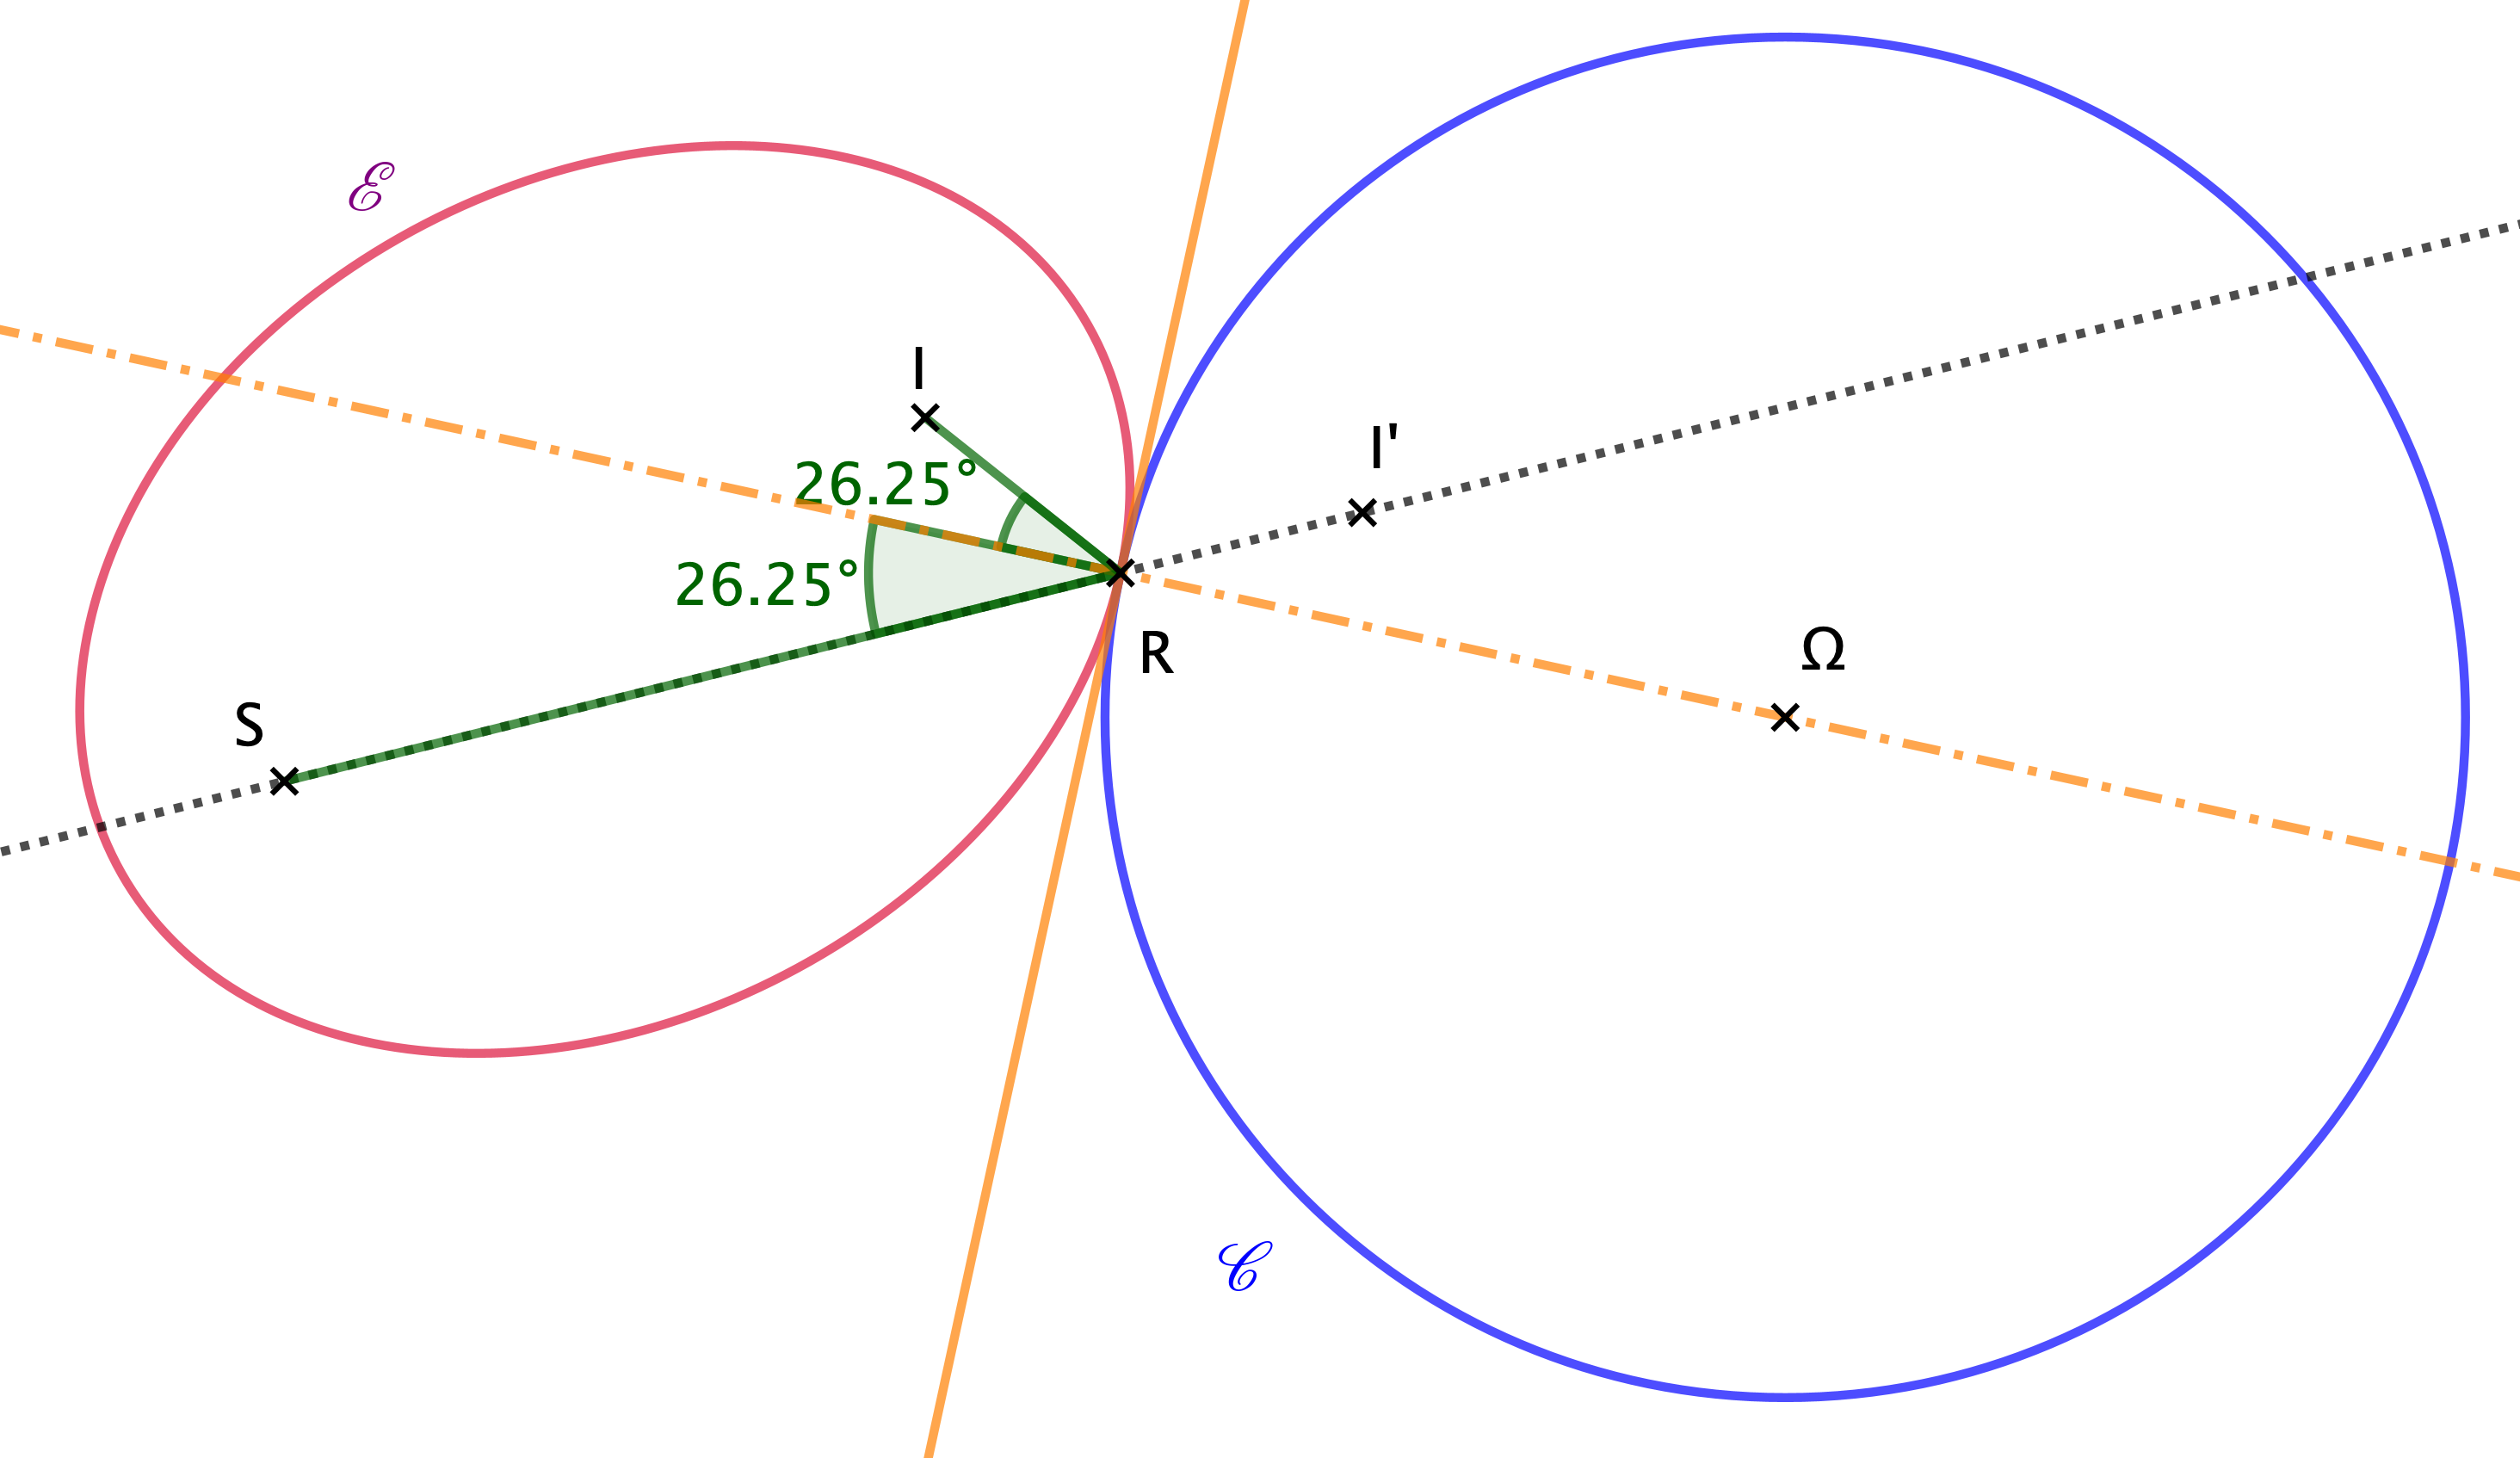
\includegraphics[scale=1.25]{ellipse.png}
\end{center}


% --------------------- %


\section{À la recherche de l'ellipse perdue}

On se place dans un repère orthonormé tel que l'on ait les faits suivantes.

\begin{itemize}[label=\small\textbullet]
	\item L'origine $O$ du repère est le milieu du segment $[SI]$ .

	\item $S\coord{1 | 0}$ et $I\coord{-1 | 0}$ .
\end{itemize}


Notant $\Omega\coord{p | q}$ , nous avons alors
$\setgeo{C} : (x - p)^2 + (y - q)^2 = r^2$
et
$\setgeo{E} : \dfrac{x^2}{a^2} + \dfrac{y^2}{b^2} = 1$ avec a minima $\coord{a | b | r} \in \big(\RRsp\big)^3$ .
On doit trouver $a$ et $b$ tels que $\card \big( \setgeo{C} \cap \setgeo{E} \big) = 1$ .


\newpage


Nous avons pour $P\coord{x | y} \in \setgeo{C} \cap \setgeo{E}$ :

\medskip

\begin{stepcalc}[style=ar*, ope=\implies]
	(x - p)^2 + (y - q)^2 = r^2
\explnext*{$\rho = r^2$}{}
	x^2 - 2 p x + p^2 + y^2 - 2 q y + q^2 = \rho
\explnext*{$\setgeo{E} : b^2 x^2 + a^2 y^2 = a^2 b^2$}{}
	a^2 x^2 - 2 p a^2 x + p^2 a^2 + (a^2 b^2 - b^2 x^2) - 2 q a^2 y + a^2 q^2 = a^2 \rho
\explnext*{$\alpha = a^2$ , $\beta = b^2$ , $\gamma = a^2 b^2$}{}
	\alpha x^2 - 2 p \alpha x + p^2 \alpha + (\gamma - \beta x^2) - 2 q \alpha y + \alpha q^2 = \alpha \rho
\explnext{}
      2 q \alpha y
    =
	  (\alpha - \beta) x^2 
	- 2 p \alpha x 
	+ \alpha(p^2 + q^2) 
	+ \gamma - \alpha \rho
\end{stepcalc}

\medskip

Nous savons que $\alpha > 0$ , mais il est aussi immédiat que la configuration proposée empêche d'avoir $q = 0$ , nous avons ensuite :

\medskip

\begin{stepcalc}[style=ar*, ope=\implies]
	\beta x^2 + \alpha y^2 = \gamma
\explnext{}
    4 q^2 \alpha \beta x^2 + 4 q^2 \alpha^2 y^2 = 4 q^2 \alpha \gamma
\explnext{}
    4 q^2 \alpha \beta x^2 
    + 
    \big(
    	(\alpha - \beta) x^2 
	- 2 p \alpha x 
	+ \alpha(p^2 + q^2) 
	+ \gamma - \alpha \rho
    \big)^2
    =
    4 q^2 \alpha \gamma
\end{stepcalc}

\bigskip

\hrule

\oldsection{AFFAIRE À SUIVRE...}

\bigskip

\hrule



%% --------------------- %
%
%
%\section{Simplification généraliste de la recherche}
%
%Il est facile de se convaincre que l'on peut supposer $p = 0$ via un bon choix de repère. Nous avons alors :
%
%\medskip
%
%\begin{stepcalc}[style=ar*, ope=\implies]
%	(\beta - \alpha) x^2 - 2 \beta m x + \beta m^2 + \alpha + \alpha p^2 - \gamma = 2 \alpha p y
%\explnext*{$p = 0$}{}
%	(\beta - \alpha) x^2 - 2 \beta m x + \beta m^2 + \alpha - \gamma = 0
%\end{stepcalc}
%
%\medskip
%
%Nous voulons une unique solution donc nous devons avoir :
%
%\medskip
%
%\begin{stepcalc}[style=ar*, ope=\implies]
%	\Delta = 0
%\explnext{}
%	4 \beta^2 m^2 - 4 (\beta - \alpha) (\beta m^2 + \alpha - \gamma) = 0
%\explnext{}
%	4 \big( \beta^2 m^2 - \beta^2 m^2 - \beta \alpha + \beta \gamma + \alpha \beta m^2 + \alpha^2 - \alpha \gamma \big) = 0
%\explnext*{$\gamma = \alpha \beta$}{}
%	- \beta \alpha + \alpha \beta^2 + \alpha \beta m^2 + \alpha^2 - \alpha^2 \beta = 0
%\explnext*{$\alpha \neq 0$ et $\beta \neq 0$}{}
%	- 1 + \beta + m^2 + \dfrac{\alpha}{\beta} - \alpha = 0
%\explnext{}
%	\bigg( 1 - \dfrac{1}{\beta} \bigg) \alpha
%	=
%	- 1 + \beta + m^2
%\end{stepcalc}
%
%% alpha_1 = (- 1 + beta_1 + x(M)^2 ) / ( 1 - 1 / beta_1 )
%
%On note ici que $\beta = 1$ donnerait $m =0$ ce qui est impossible car $p = 0$ . Tentons notre chance avec une valeur de notre choix de $\beta \neq 1$ dans l'exemple suivant.


\end{document}

